\documentclass[openany,oneside,notitlepage]{book}
\usepackage{graphicx}
\usepackage[utf8]{inputenc}
\usepackage[italian]{babel}
\usepackage{fancyhdr}
\usepackage{eurosym}
\usepackage{hyperref}
\pagestyle{fancy}
\renewcommand{\chaptermark}[1]{\markboth{#1}{}}
\renewcommand{\sectionmark}[1]{\markright{#1}{}}
\renewcommand{\chaptername}{}
\fancyhf{}
%\fancyhead[LE,RO]{\mdseries\thepage}
\fancyhead[LO,LE]{\mdseries\rightmark}
\fancyhead[RO,RE]{\mdseries\leftmark}
\cfoot{\thepage}
\renewcommand{\headrulewidth}{0.5pt}
\renewcommand{\footrulewidth}{0pt}
\addtolength{\headheight}{0.5pt}
\addtolength{\headwidth}{1cm}
%% \addtolength{\textheight}{4cm}
%% \addtolength{\textwidth}{1cm}
%\setlength{\marginparwidth}{4.5cm}
\setlength{\parindent}{0pt}
\setlength{\parskip}{0pt}
%% \addtolength{\voffset}{-2cm}
%% \addtolength{\hoffset}{-2cm}
%% \addtolength{\hoffset}{-1cm}
\linespread{1}%interlinea
\setlength{\marginparwidth}{4.5cm}
\setlength{\parindent}{0pt}
\setlength{\parskip}{0pt}
\title{Entropia in Musica}
\author{Giovanni Marelli}
\date{Salò \today}
\begin{document}
\pagestyle{fancy}
%\maketitle
\section{Entropia come misura di creatività}
\begin{equation} E = -\sum_i p_i\log p_i \end{equation}
Per ogni midi considero l'informazione contenuta nel ritmo, nell'escursione e quella totale.
Calcolo quindi gli istogrammi relativi alla durata della nota, al timbro e nota e timbro separatamente.
\begin{table}[!h]
\centering
\begin{tabular}{c c c c}
Pezzo & ritmica& cromatica & totale \\
Flutto & 2.024 & 5.239 & 6.56 \\
\end{tabular}
\end{table}
 Calcolo le distanze relative tra i pezzi: \\
 \begin{equation} d_{ij}^2 = (E_i^r-E_j^r)^2 +  (E_i^c-E_j^c)^2 +  (E_i^t-E_j^t)^2 \end{equation}
 e costruisco il grafo per i pezzi la cui distanza è minore di 0.5 utilizzando il database neo4j.\par
\begin{verbatim}
CREATE (Entropy:Measure {label:'measure for creativity'})
CREATE (Aere:Song { id:'0', name:'Aere', entropy:'4.962'})
CREATE (AjdeJano) - [:DIST{d: 0.470}] -> (Prolecic),
\end{verbatim}
\begin{figure}[!h]
\centering
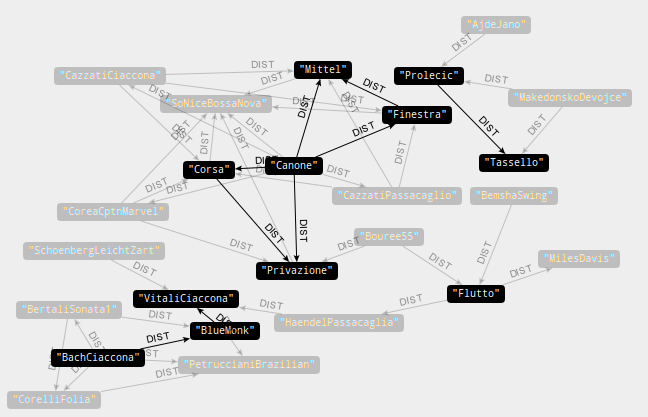
\includegraphics[width=13cm]{DistCanzoni}
\end{figure}
ed ecco svelate le fonti\ldots\\
L'evoluzione dell'entropia si arresta arresta oltre un certo tempo ed in alcuni casi diminuisce.\par\par
\begin{figure}[!h]
\centering
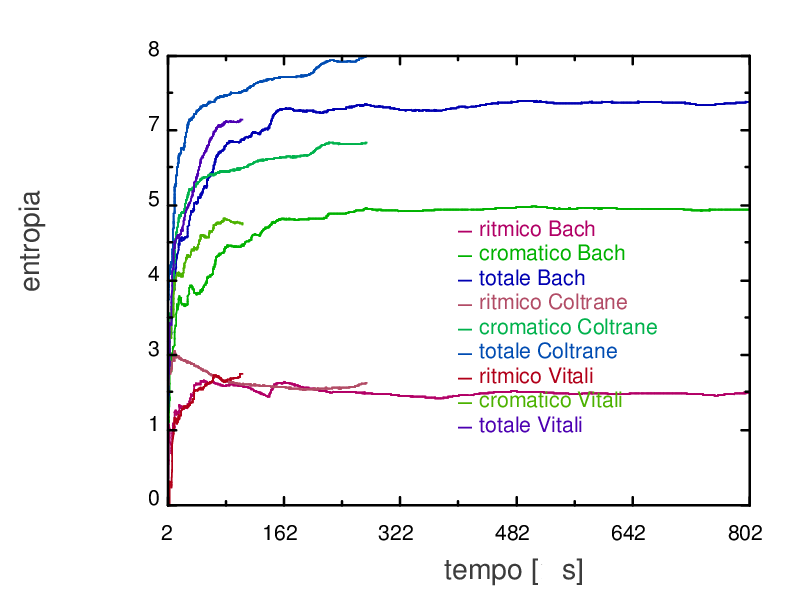
\includegraphics[width=13cm]{EntropyEvolution}
\end{figure}
Nel grafico, ciaccona di Bach, lazy bird di Coltrane, ciaccona di Vitali. \par
\vspace{\stretch{1}}
%% \begin{minipage}{.8\textwidth}
%% \end{minipage}
%% \begin{minipage}{.2\textwidth}
\begin{figure}[!b]

\includegraphics[width=2cm]{Licenco}
\end{figure}
%% \end{minipage}
\end{document}
